%!TeX root=../tese.tex
%("dica" para o editor de texto: este arquivo é parte de um documento maior)
% para saber mais: https://tex.stackexchange.com/q/78101

\chapter{Metodologia}

% falar sobre validação cruzada
% falar que foi em python, libs, 
% dados amostrados ao longo do tempo => não misturamos 
% validação cruzadas 
% n modelo => falar melhores

% melhorar.. só usar isso?

Nesta seção é feito um detalhamento dos dados utilizados que 
abrange as fontes e as estratégias de preparação e de pré-processamento. 
Também são descritas as 
tecnologias utilizadas na implementação, as métricas estatísticas 
usadas para mensurar o desempenho dos modelos e o método de validação
cruzada aplicado na avaliação dos modelos.

\section{Tecnologias utilizadas}

Este projeto foi implementado na linguagem Python e 
utilizando o ambiente de desenvolvimento interativo fornecido pelo Jupyter.
Foram utilizadas as bibliotecas Pandas e NumPy para realizar a preparação dos dados,
além da TensorFlow e Scikit-learn com o intuito de treinar e avaliar os modelos.
A maior parte dos gráficos foram gerados por meio das bibliotecas 
Seaborn e Matplotlib, contudo alguns foram contruídos por meio da plataforma
Microsoft Excel.

Os códigos utilizados no projeto estão disponíveis em \url{https://github.com/LeiteJu/TCC}.

\section{Dados}
\label{sec:dados}

Os algoritmos de aprendizado de máquina utilizam dados para fazer 
previsões. 
Neste trabalho, optou-se por utilizar dados de 2003 até 2019 para treinamento e 
avaliação dos modelos, em virtude da disponibilidade dos dados de consumo mensal 
de cimento. Além disso,
adotou-se granularidade de dados
mensal e por estado com o intuito de aumentar a quantidade de entradas disponíveis 
para treinamento e avaliação dos modelos\footnote{Por exemplo, se fossem usados dados 
anuais a nível de estados da União, haveria 459 \textit{inputs} para os modelos, ao 
utilizar dados mensais por estado, o número de entradas disponíveis aumenta para 5508.}.
Essa estratégia de aumentação de dados visa diminuir o risco de  
\textit{underfitting}, que acontece quando o 
modelo não é capaz de aprender com os dados e resulta em altos erros nas etapas de
treinamento e teste, de acordo com \citet{Goodfellow-et-al-2016}.


\subsection{Fontes}

O modelo utiliza dados econômicos, sociais e da construção
civil para estimar a demanda por cimento. Na tabela
\ref{tab:indicadores}, são
apresentados os dados utilizados, juntamente com a fonte, a granularidade e o período em que os dados 
estavam disponíveis.


\begin{table}[H]
    \centering
    \caption{Indicadores utilizados no trabalho}
    \begin{tabular}{llll}
        \toprule
        Dado                   & Fonte & Período disponível & Granularidade         \\
        \midrule
        PIB a preços constantes     
                                    & IBGE\footnote{\label{portal ipea} Dado retirado do portal do Ipeadata em \url{http://www.ipeadata.gov.br/Default.aspx}}  & 1983 até 2019      & anual por estado      \\
        PIB a preços de mercado      & IBGE\footref{portal ipea}  & 1985 ate 2019      & anual por estado      \\
        PIB \textit{per capita}              & IBGE\footref{portal ipea}  & 1985 até 2019      & anual por estado      \\
        PIB da construção civil      & IBGE\footref{portal ipea}  & 1985 até 2019      & anual por estado      \\
        Desemprego                   & IBGE\footref{portal ipea}  & 1991 até 2022      & irregular \footnote{Havia dados de 1992 até 2014
        com granularidade anual e por estado. A partir de 2012 foram disponibilizados dados mensais a nível de Brasil por conta da 
        Pesquisa Nacional por Amostra de Domicílios (PNAD) Contínua mensal realizada pelo IBGE. Neste trabalho, utilizou-se os dados anuais até 2012
        e, após 2012, os dados provenientes da PNAD Contínua.} \\
        IPCA                        & IBGE\footnote{Dado retirado do IBGE em \url{https://sidra.ibge.gov.br/tabela/1737}}  & 1981 até 2021      & mensal para o Brasil      \\
        INCC                        & FGV\footnote{Dado obtido a partir do portal da FGV em \url{https://www.debit.com.br/tabelas/tabela-completa-pdf.php?indice=incc}}   & 1980 ate 2021      & mensal para o Brasil      \\
        IGP                         & FGV\footref{portal ipea}   & 1944 até 2021      & mensal para o Brasil      \\
        Taxa Selic                  & IBGE\footnote{Dado obtido em \url{https://www.debit.com.br/tabelas/tabela-completa.php?indice=selic}}  & 1986 até 2022      & mensal para o Brasil      \\
        NFSP                        & BACEN\footref{portal ipea}  & 1991 até 2022      & mensal para o Brasil      \\
        Estoque líquido de capital fixo   & IPEA\footref{portal ipea}   & 1947 ate 2019      & anual para o Brasil      \\
        População                   & IBGE\footnote{Dado obtido do portal Base dos Dados em \url{https://basedosdados.org/dataset/br-ibge-populacao}}   & 1991 até 2021      & anual por estado      \\
        IDH                         & IBGE\footref{portal ipea}   & 1991 ate 2017      & irregular\footnote{Os indicadores de IDH (Renda, Longevidade e Educação) estão disponíveis a nível de estados da União em anos de censo do IBGE (1990, 2000, 2010). Há 
        dados, também, de 2014 a 2017 por conta da PNAD Contínua.}      \\
        Produção mensal de cimento  & SNIC\footnote{\label{cbic} Dados retirados do portal \url{http://www.cbicdados.com.br/menu/materiais-de-construcao/cimento}}  & 2003 até 2022      & mensal por estado      \\
        Valor médio do cimento\footnote{Evolução do valor médio/mediano do cimento Portland 32 em US\$/Tonelada}      & SNIC\footref{cbic}   & 1947 ate 2019      & anual para o Brasil      \\
        Consumo de cimento em ton.  & SNIC\footref{cbic} & 2003 até 2019 & mensal por estado \\
        \bottomrule
    \end{tabular}
    \label{tab:indicadores}
\end{table}
% quem sabe por a legenda no apendice

Na tabela, são utilizadas siglas 
para melhorar a legibilidade, uma descrição das abreviações utilizadas no 
trabalho pode ser encontrada no início do documento, em Lista de Abreviaturas.

\subsection{Preparação dos dados}

Com o intuito de direcionar a estratégia de preparação de dados,
foi realizada uma análise exploratória dos dados de 
entrada e da variável resposta. 
Foi identificada nessa análise, uma alta
taxa de variação dos atributos,
dessa forma, está presente nos dados um grande número de \textit{outliers}.
De acordo com \citet{outliers} e \citet{tukey77}, \textit{outliers} são
observações discrepantes do restante dos dados
que podem interferir no processo de previsão. 

Um exemplo de atributo com alta variação é o PIB da contrução civil,
que apresenta desvio padrão maior que o valor médio dessa variável.
Para ilustrar a distribuição dos pontos de dados desse indicador, utiliza-se 
um gráfico \textit{boxplot} na figura \ref{fig:boxplot_pibcc}.

\begin{figure}[H]
    \centering
    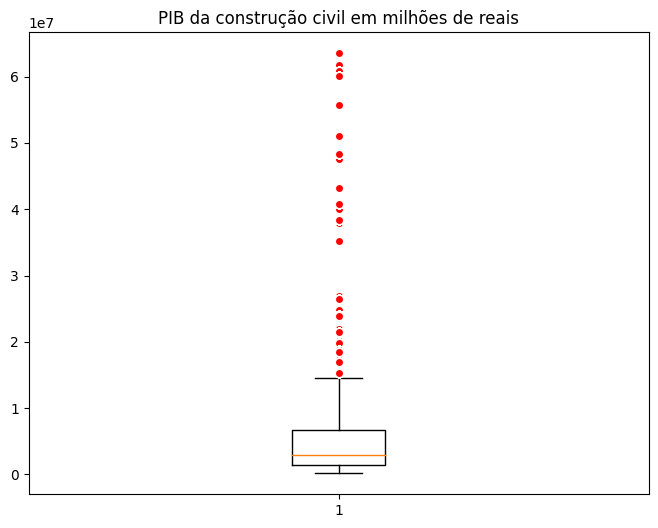
\includegraphics[width=9cm]{../figuras/graficos/boxplot-pib-cc.png}
    \caption{Gráfico \textit{boxplot} do PIB da construção civil}
    \label{fig:boxplot_pibcc}
\end{figure}

Segundo \citet{boxplot}, o \textit{boxplot} é
uma técnica estatística utilizada para identificar visualmente padrões nos dados. 
Na figura acima, a linha em laranja corresponde à mediana \footnote{Mediana é
valor que fica no meio quando os dados estão ordenados ou a média
dos dois valores centrais se o número de pontos de dados for par.
(\cite{boxplot-stat})} 
dos dados, os limite inferior e o superior ao retângulo representam
o primeiro e terceiro quartis\footnote{O primeiro quartil marca a mediana 
relativa aos valores superiores à mediana destacada na imagem. O terceiro quartil,
de maneira análoga, assinala a mediana dos valores inferiores à mediana destacada. 
Assim, entre o primeiro e terceiro quartis está contida metade
dos dados.}, respectivamente. As observações fora do intervalo dos limites 
superior e inferior, representadas com círculos vermelhos na figura, são 
\textit{outliers}. Pode-se observar, então, a alta incidência de dados discrepantes
nesse indicador.

Parte do alto volume de \textit{outliers} nos atributos se deve às diferenças
econômicas, geográficas e sociais entre os estados do Brasil. A saber, o valor 
médio do PIB da construção civil no estado 
de São Paulo é de $48,96$ milhões, enquanto em Santa Catarina é de $7,1$ milhões e 
em Roraima, de $0,4$ milhões. Aliás, ao analisar o PIB da construção civil nas 
regiões do país, há uma significativa redução no número de dados discrepantes, como 
pode-se observar na figura abaixo.

\begin{figure}[H] 
    \centering
    \begin{subfigure}{5cm}
      \centering 
      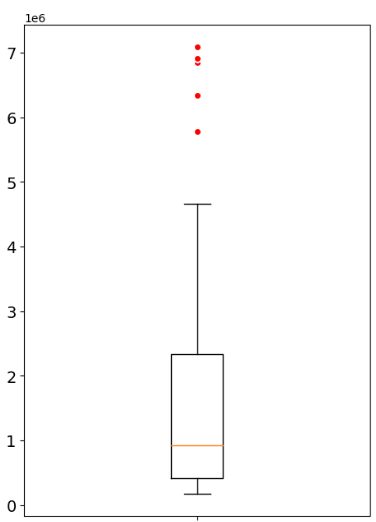
\includegraphics[width=4.5cm]{../figuras/graficos/boxplot-pib-cc-n.png}
      \caption{Região Norte}
      \label{fig:boxplot-n}
    \end{subfigure}
    \hfill 
    \begin{subfigure}{5cm}
        \centering 
        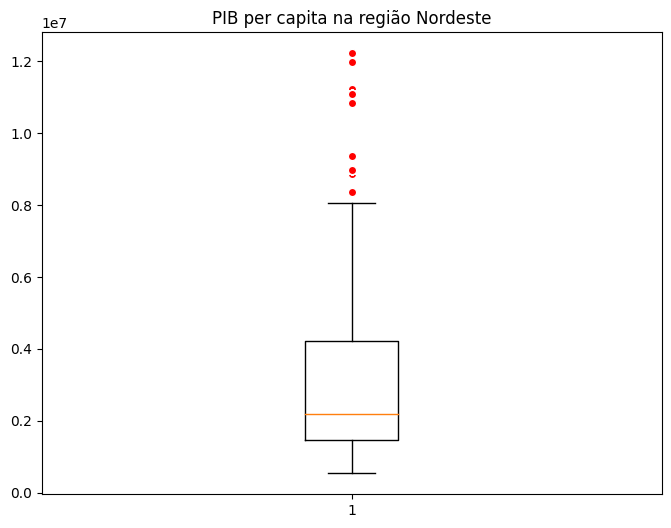
\includegraphics[width=4.5cm]{../figuras/graficos/boxplot-pib-cc-ne.png}
        \caption{Região Nordeste}
        \label{fig:boxplot-ne}
    \end{subfigure}
    \begin{subfigure}{5cm}
        \centering 
        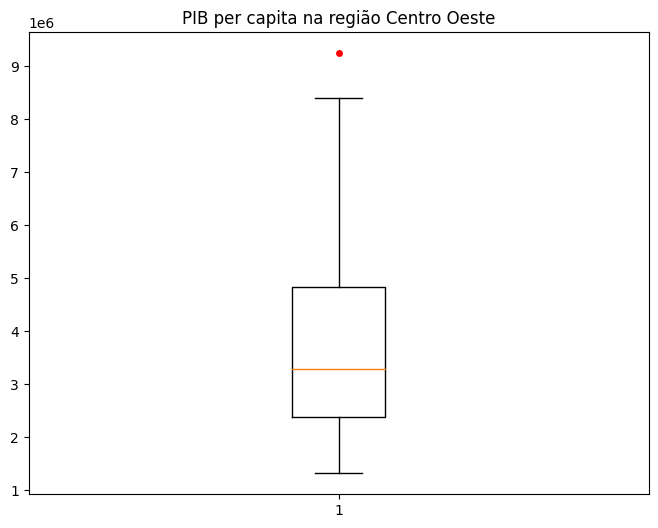
\includegraphics[width=4.5cm]{../figuras/graficos/boxplot-pib-cc-co.png}
        \caption{Região Centro Oeste}
        \label{fig:boxplot-co}
    \end{subfigure}
    \begin{subfigure}{5cm}
        \centering 
        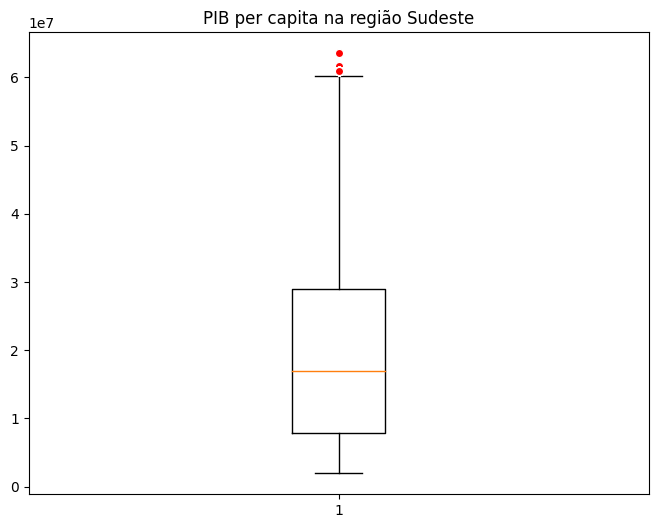
\includegraphics[width=4.3cm]{../figuras/graficos/boxplot-pib-cc-se.png}
        \caption{Região Sudeste}
        \label{fig:boxplot-se}
    \end{subfigure}
    \begin{subfigure}{5cm}
        \centering 
        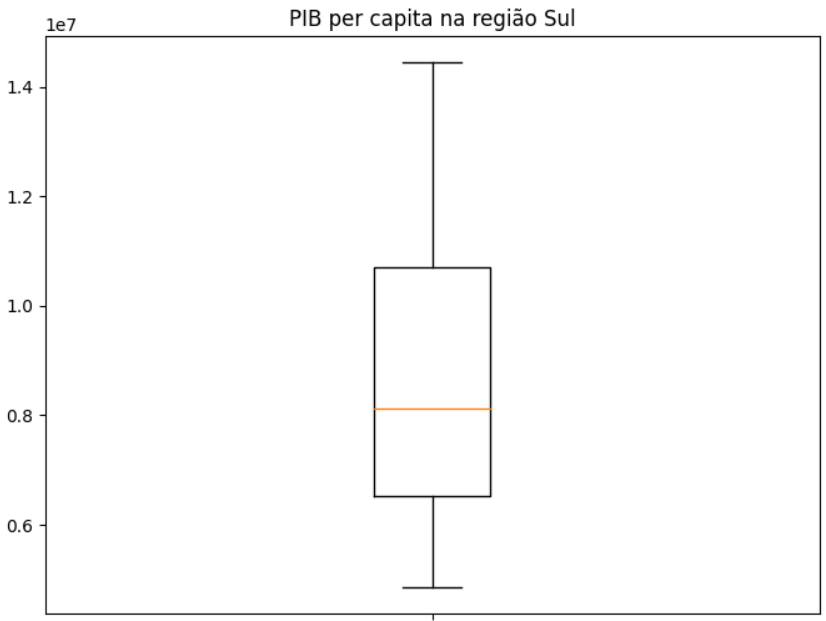
\includegraphics[width=4.5cm]{../figuras/graficos/boxplot-pib-cc-s.png}
        \caption{Região Sul}
        \label{fig:boxplot-s}
    \end{subfigure}
    \caption{Comparação dos gráficos \textit{boxplot} entre as regiões}
  \end{figure}

Além disso, analisou-se, a correlação entre as variáveis de entrada com o auxílio 
de uma matriz de correlação. Foi identificada
alta correlação entre os indicadores do PIB do estado, o PIB da construção
civil e a população. Além disso, há correlação entre os três indicadores
de IDH (Longevidade, Saúde e Renda) e entre o preço do saco de cimento e o preço do kilograma, como pode-se
validar na figura \ref{fig:matriz-corr}.

\begin{figure}[H]
    \centering
    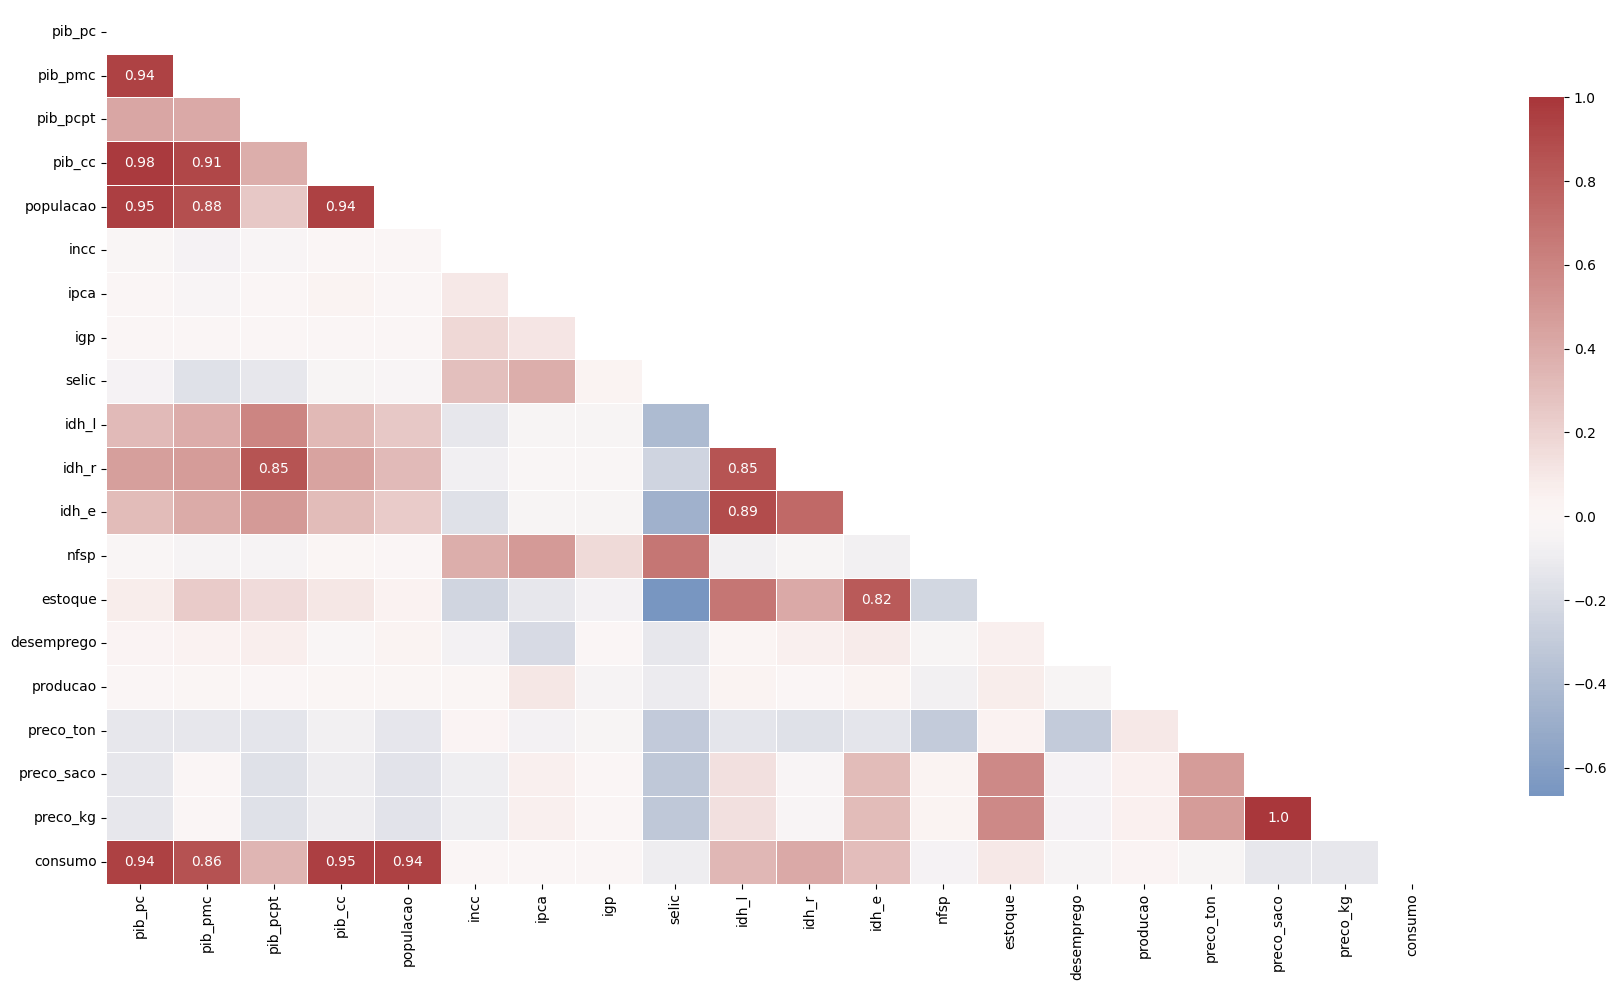
\includegraphics[width=13cm]{../figuras/graficos/matriz-corr.png}
    \caption{Matriz de correlação}
    \label{fig:matriz-corr}
\end{figure}

Foram adotadas estratégias para garantir dados na granularidade
mensal e por estado. Caso os indicadores apresentassem granularidade anual, o valor de
cada medição foi dividido por 12 de modo a obter a média mensal utilizada em 
todos os meses do ano correspondente. Caso a granularidade
fosse a nível de Brasil, o valor apresentado foi repetido para todos os 
estados no mês e ano correspondente. As exceções foram os 
indicadores de IDH por apresentarem valores apenas em anos específicos, conforme 
detalhado em \ref{tab:indicadores}. Nesse caso, quando não havia dados para um 
determinado ano foi repetido o valor da última medição.

Também foi necessário lidar com dados faltantes, o método utilizado foi
repetir o último valor disponível nos dados de entrada para
preencher a ocorrência faltante. Contudo, para a produção mensal de cimento e os 
indicadores de evolução do preço do cimento foi utilizado um valor não 
presente no intervalo dos dados de entrada (-1) para marcar as ocorrências 
faltantes como nulo, uma vez que essas variáveis não apresentavam 
valores mais antigos.

Além disso, foi realizado um deslocamento nos dados para garantir que a previsão
do consumo em um mês só utilize dados dos meses anterior e não do mês alvo da
previsão. atentou-se para evitar que a previsão fosse 
realizada com os dados do mês anterior ou do ano anterior no caso dos
indicadores anuais. Deslocou-se, portanto, os dados de entrada 
para frente em um ocorrência de modo a associar os dados de um 
mês com o consumo no mês seguinte.\footnote{os dados correspondentes 
a, por exemplo, fevereiro de 2004 estão relacionados ao consumo de 
cimento em março de 2004, com o objetivo de propor um cenário mais pertinente, 
uma vez que o objetivo do projeto é prever a demanda por cimento no mês seguinte 
em um estado a partir dos dados do mês atual e, eventualmente, dos anteriores.
}

Por fim, o estado correspondente à medição foi usado como dado de entrada. 
Como os modelos de inteligência artificial aceitam apenas caracteres numéricos,
utilizou-se o método de codificação \textit{one hot} para criar 27 colunas, uma
para cada estado, nas quais o valor é 1 quando a linha possui dados daquele estado 
e é 0 caso contrário.


\subsection{Pré-processamento de dados}
\label{sec:norm_dados}


\subsubsection{Normalização}



O objetivo da normalização dos dados, é garantir que as variáveis de entrada 
estejam na mesma escala. Esse processo é necessário não apenas para realizar melhor comparação entre variáveis 
com diferentes unidades, mas também para o melhor funcionamentos dos algoritmos 
de aprendizado, uma vez que se as \textit{features} estiverem em escalas diferentes
alguns pesos podem ser atualizados mais rápidos que outros. (\cite{Raschka})


A normalização garante que as variáveis de entrada estejam em uma 
escala com as propriedades de uma distribuição normal, ou seja, média ($\mu$)
igual a zero e variância ($\sigma$) igual a um. Dessa forma, a operação 
realizada para aplicar o processo em um entrada $x$ é

\begin{equation}
  z = \frac{x - \mu}{\sigma}
\end{equation}

\subsubsection{\textit{Min-Max scaler}}

O \textit{min-max scaler} transforma os dados de modo que a 
escala dos dados tenha um itnervalo definido, em geral, entre
0 e 1.

\begin{equation}
  X_{norm} = \frac{X - X_{min}}{X_{max} - X_{min}}
\end{equation}




\section{Avaliação de performance}

Para comparar a eficiência dos modelos mede-se os erros de 
cada previsão, ou seja, a distância entre o valor previsto 
pelo algoritmo e o valor do dado real. Neste trabalho, 
utilizou-se as seguintes métricas estatísticas para 
mensurar o desempenho: \textit{mean absolute error} (MAE),
\textit{root mean square  error} (RMSE) e \textit{mean 
absolute percentage error} (MAPE). Além disso, foi utilizado
o delta percentual ($\Delta$) para avaliar se o modelo tende 
a subestimar ou superestimar o valor previsto, se é otimista
ou pessimista.

\subsection{Mean absolute error (MAE)}

    O MAE, sigla do inglês para \textit{mean absolute error}
    ou média do erro absoluto mede o erro absoluto de cada previsão
    e é dado por:\cite{forecast-evaluation-ds}

    \begin{equation}
        MAE = \frac{\sum_{i=1}^n |\hat{y}_i - y_i|}{n}
    \end{equation}

\subsection{Root mean squared error (RMSE)}

    A RMSE, sigla para \textit{root mean squared  error} é
    semelhante à MAE, contudo eleva os erros ao quadrado antes de 
    somá-los e tira a raiz logo depois. A RMSE é, portanto, 
    mais sensível a \textit{outliers}.\cite{forecast-evaluation-ds}

    \begin{equation}
        RMSE = \sqrt{\frac{\sum_{i=1}^n (\hat{y}_i - y_i)^2}{n}}
    \end{equation}

\subsection{Mean absolute percentage error (MAPE)}

    Foi utilizada também a MAPE, \textit{Mean absolute
    percentage error}, para mensurar a escala do erro em 
    relação ao tamanho das medições.

    \begin{equation}
        MAPE=\sum_{t=1}^n\left|\frac{y_t-\hat{y}_t}{y_t}\right|
    \end{equation}

\subsection{Variação percentual}

A variação percentual, $\Delta$, é utilizado para mensurar se o 
modelo apresenta tendência de subestimar ou superestimar a variável, se 
é otimista ou pessimista.

\begin{equation}
    \Delta = \frac{\hat{y_i} - y_i}{y_i}
\end{equation}

